% Data and estimation of signal

Data is downloaded from OptionMetrics, CRSP, Kenneth French's Library and Open Asset Pricing. The extensive data has been filtered to only include the stocks registered on American exchanges. And they are only included in the portfolio formation if a signal is observed in the relevant period, which is the preceding week. All data have been joined together using the SECIDs and PERMNOs.

Wharton's Research Database has option data available through OptionMetrics on a daily basis from the first of January 1996 until December 31st 2021 (as of 1st of May 2023). Center for Research in Security Prices has data available through the same accesspoint with daily holding period returns for all stocks registered in the US. To compliment the portfolios formed based on the implied volatility spread, I have included portfolios formed on size and value by Kenneth French\footnote{The data is available at his webpage: \url{http://mba.tuck.dartmouth.edu/pages/faculty/ken.french/data_library.html}.} as well as some of the factors calculated both with a daily frequency and a weekly frequency. To compliment the factors already retrieved from French, I also include selected factors available from Open Asset Pricing \citep{chen_zimmermann}. 

The risk free rate deployed to get excess returns is the 1-month t-bill rate supplied on a daily basis in Kenneth French's Library. 

The returns of each stock can be calculated in different ways. The first approach is to use the supplied opening price and closing price of each stock at each day, and the second approach is to use the holding period return supplied in the dataset as well. I have chosen the second option, as this takes any stocksplits or dividend payouts into account. This can clearly be seen in Figure \ref{fig:crspreturns_openclose_vs_ret}, where six representative sample years are plotted with all daily returns as calculated through the two different approaches. Note that the axes are different, and if these two methods were equal, the observations would lie on a perfect line of $x=y$ (which they clearly do not).

The conditions for excluding some of the data regarding the implied volatilities are introduced in \cite{cremers2010deviations}. The conditions are elaborated below. Note, however, that as also discussed in \cite{shang2016option}, I will do the analysis for a dataset with the conditions imposed, but also include the results from the analysis without the conditions imposed in the appendix, to show the effect of the conditions and the robustness of the results. 

The signal is the spread between the implied volatility of call and put options with the same maturity and strike. These values are observed at market close at a daily frequence. I will take an average across maturities and strikes everyday for each stock to have a simple signal. This average can both be a simple average across every available datapoint or a weighted average using the open interest reported at market close for each pair. \cite{cremers2010deviations} argue that the latter approach incorporates the liquidity aspect of the options. I assume that the more liquidity an option has, the more fair is the price, and the more reflective of the market's opinion is it. Thus the latter approach for weighting the implied volatility spread ensures that the signal incorporates the market's view.

\textbf{Conditions} The conditions for including the options in the signal formation is described below. The first condition is in regards to the implied volatility of each option. These conditions are not related to the definition of the following unconditional and conditional analysis. 

\begin{mycondition}{Restrictions on Implied Volatility Level}{condition:implvol}
	$$ 0 \leq IV_{j,t}^{i,call} \leq 1.5\; \text{and} \; 0 \leq IV_{j,t}^{i,put} \leq 1.5 $$
	
	The implied volatility should be within these limits for both puts and calls for the spread to be included in the signal, which naturally limits the distribution of the implied volatility spread.
	The historical volatility of the stock markets represented by the VIX Index reached a max of 0.7 in 2017, therefore a limit of 1.5 on individual options is sensible. 
\end{mycondition}

The second condition relates to the time to maturity of the option pairs, measured in days.

\begin{mycondition}{Restrictions on Time To Maturity}{condition:ttm} 
	$$7 \leq TTM_{days}  \leq 365 $$
	
	Options with time to maturity within these limits are the most liquid and by excluding the imminent maturing options, the signal will only contain data on options with maturity prevailing the return period.
\end{mycondition}

For the last condition, the forward price of the stock is estimated at the point of daily closing prices for the individual option. Optionmetrics describes the calculation as follows: "The forward security price is calculated based on the last closing security price, plus the interest, less projected dividends" - \cite{optionmetrics} and the standard form of the equation is given in Equation \ref{eq:forwardprice}.

\begin{mycondition}{Restrictions on Moneyness}{condition:moneyyy}
	$$ 0.7 \leq \frac{F_{0,i}}{K} \leq 1.3 $$
	
	The moneyness (ratio between forward price of the underlying stock and the strike price of the option) should be between those limits, which ensures that the options included are somewhat close to being at-the-money and decreases the noise from illiquid deep-in-the-money or deep-out-of-the-money options.
\end{mycondition}


The average of these is taken per day, and the observed signal for return predictability is the latest day within the last 7 days before the return period begins. If there is no observed spread in this period, the stock is not considered for portfolio formation.

\textbf{Signals Deployed} The two main signals formed on the data are the actual average value of the implied volatility spread and the recent change in the implied volatility spread for each individual stock. 

The subsample of relevant options and stocks will be formed to fulfill the above-mentioned conditions. Furthermore, as each stock has multiple pairs of put-calls and therefore also multiple implied volatility spreads observed each day across maturities and strikes, I have two subsample regarding either a weighted mean of these implied volatility spreads using the sum of open interest, and a subsample with just a simple mean of all these values. The difference in the distribution of these means across the time period seems rather stationary. In Figure \ref{fig:distribution_of_signal_entire_period} I show the median, 95\% and 5\% percentile of each of these subsamples across the entire sample period. Thus I note that the signal seems very stationary, and that prominent outliers are present in all four subsample with (C) having the most volatile median and (A) having more volatile percentiles. 

It is interesting to investigate these plots, as they show very little difference between them, and as such, it seems an arbitrary choice to filter out the option pairs, unless the economic arguments are convincing. Furthermore, a weighting according to the open interest is also argued for by \cite{cremers2010deviations} and likewise deployed in \cite{shang2016option}. Some of the most prominent results will therefore also be reported for each of these subsamples, to investigate the effect from making these choices. 

To calculate the second signal, I take the difference of the earliest reported average implied volatility spread and the latest reported value within a subsample of the last seven days before portfolio formation. Thus a change is reported and used for sorting portfolios. I believe this signal to be more informative and relevant in a combination with the value of the implied volatility spread and not a suitable candidate signal for univariate portfolio sorting. The reasoning is based on the object of this project to find a signal to proxy for the risk associated with mispricing of options, especially related to the too-high priced put options on stocks which might proxy some loss aversion mechanics on the stock market, and as such, I am not interested in how this mispricing changes week-on-week only, but it is relevant when combined with the value of the implied volatility spread.

\textbf{Metadata} Different measures of metadata are plotted in Figure \ref{fig:data_metadata}. These plots show the evolution of some metrics across the sample period. In general most of the data has increased over the sample period, and a  picture of effect from the IT-bubble in the early 2000's, the financial crisis in 2008 and the COVID-19 shock and subsequent upward trend following.

COMMENT MORE HERE

\begin{figure}
	\centering
	\caption[Metadata, CRSP and OptionMetrics]{Volume traded, Number of Firms and Median bid-ask spread for CRSP and OptionMetrics}
	
	\begin{tabular}{ccc}%c}
		\subfloat[OptionMetrics : Open Interest and Volume across two subsamples]{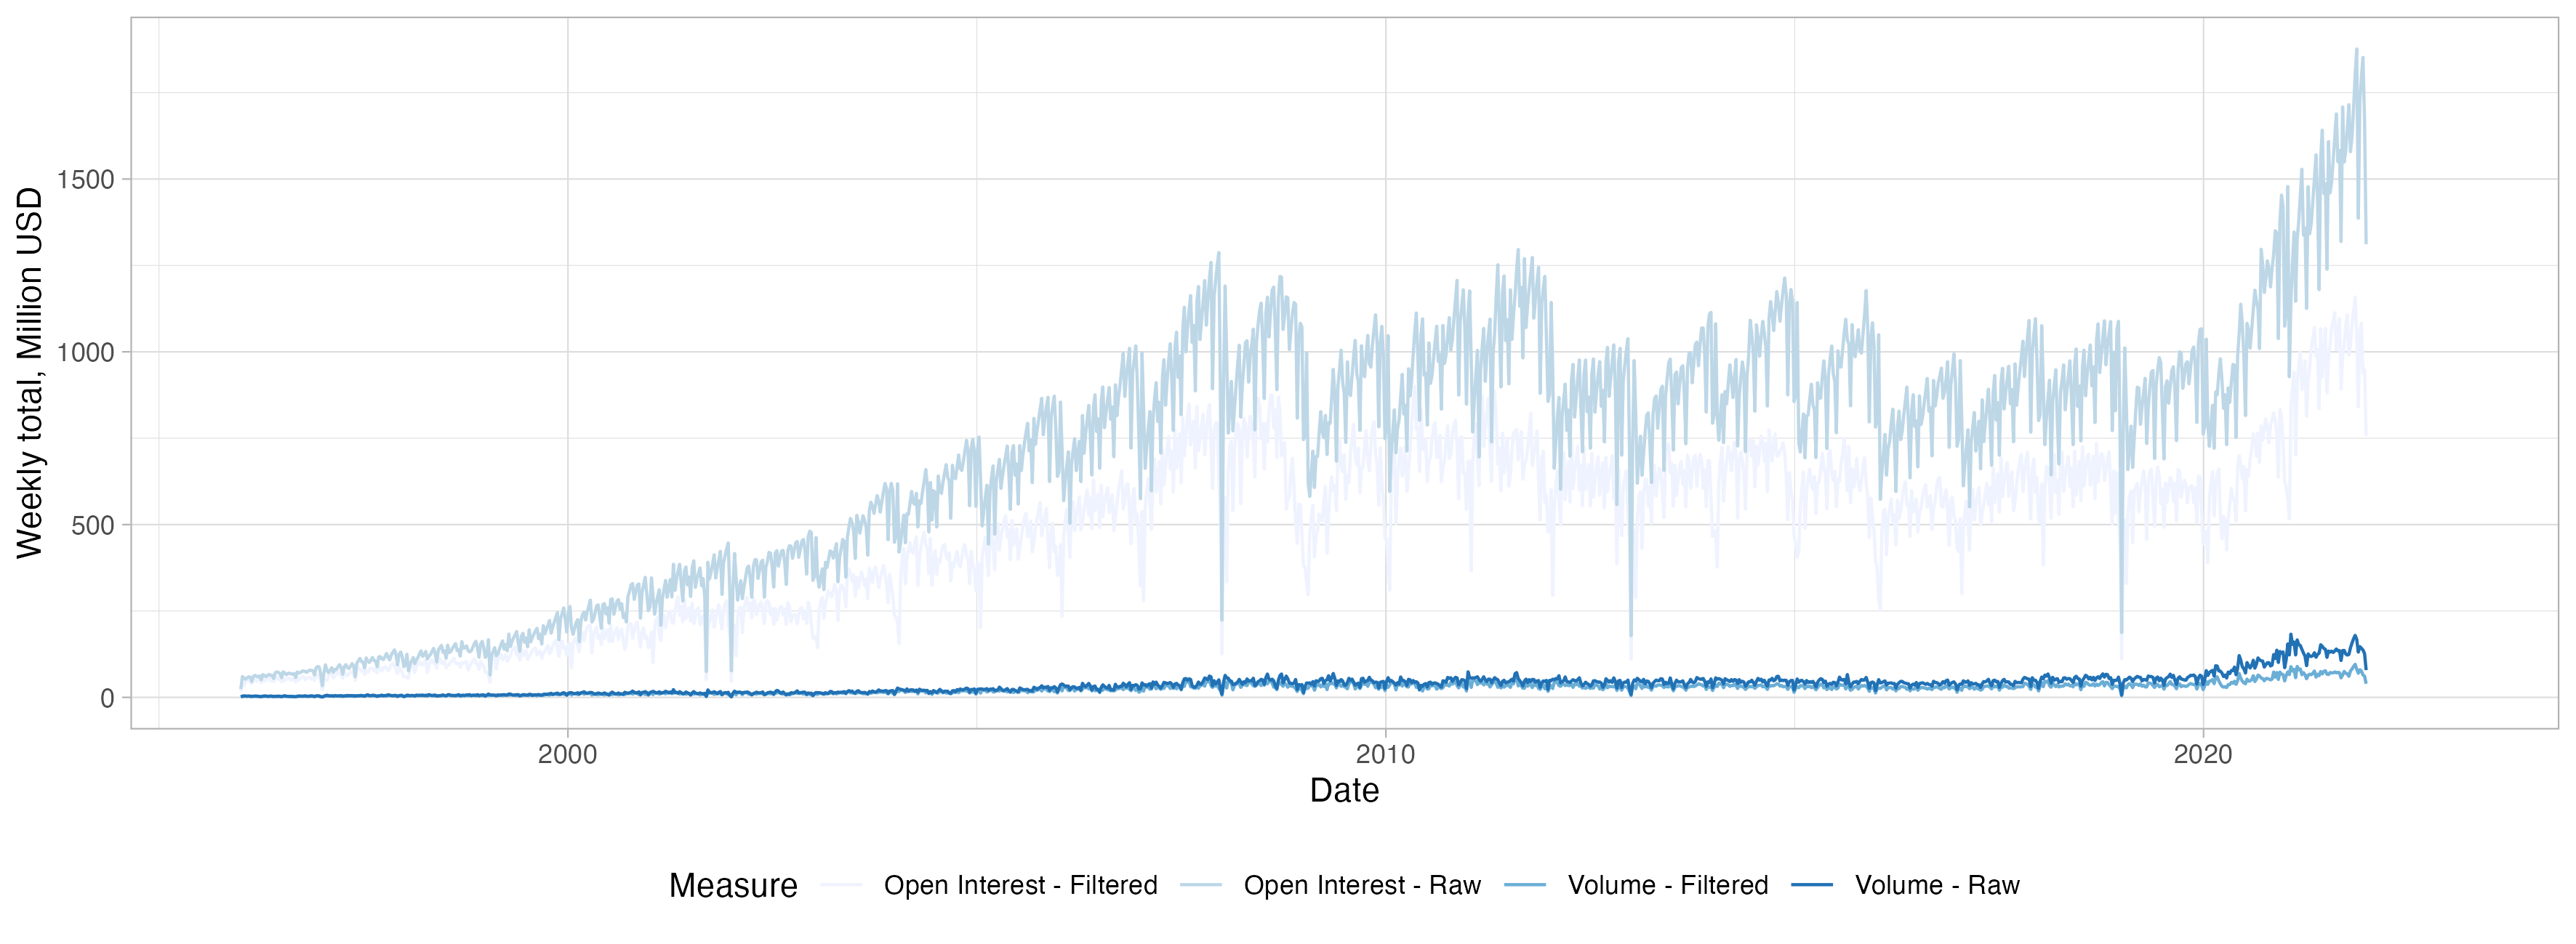
\includegraphics[width=0.85\textwidth]{./Plots/metadata_optionm_openinterestVol_entireperiod.png}} \\
		\subfloat[CRSP : Volume Traded and total Market Value ]{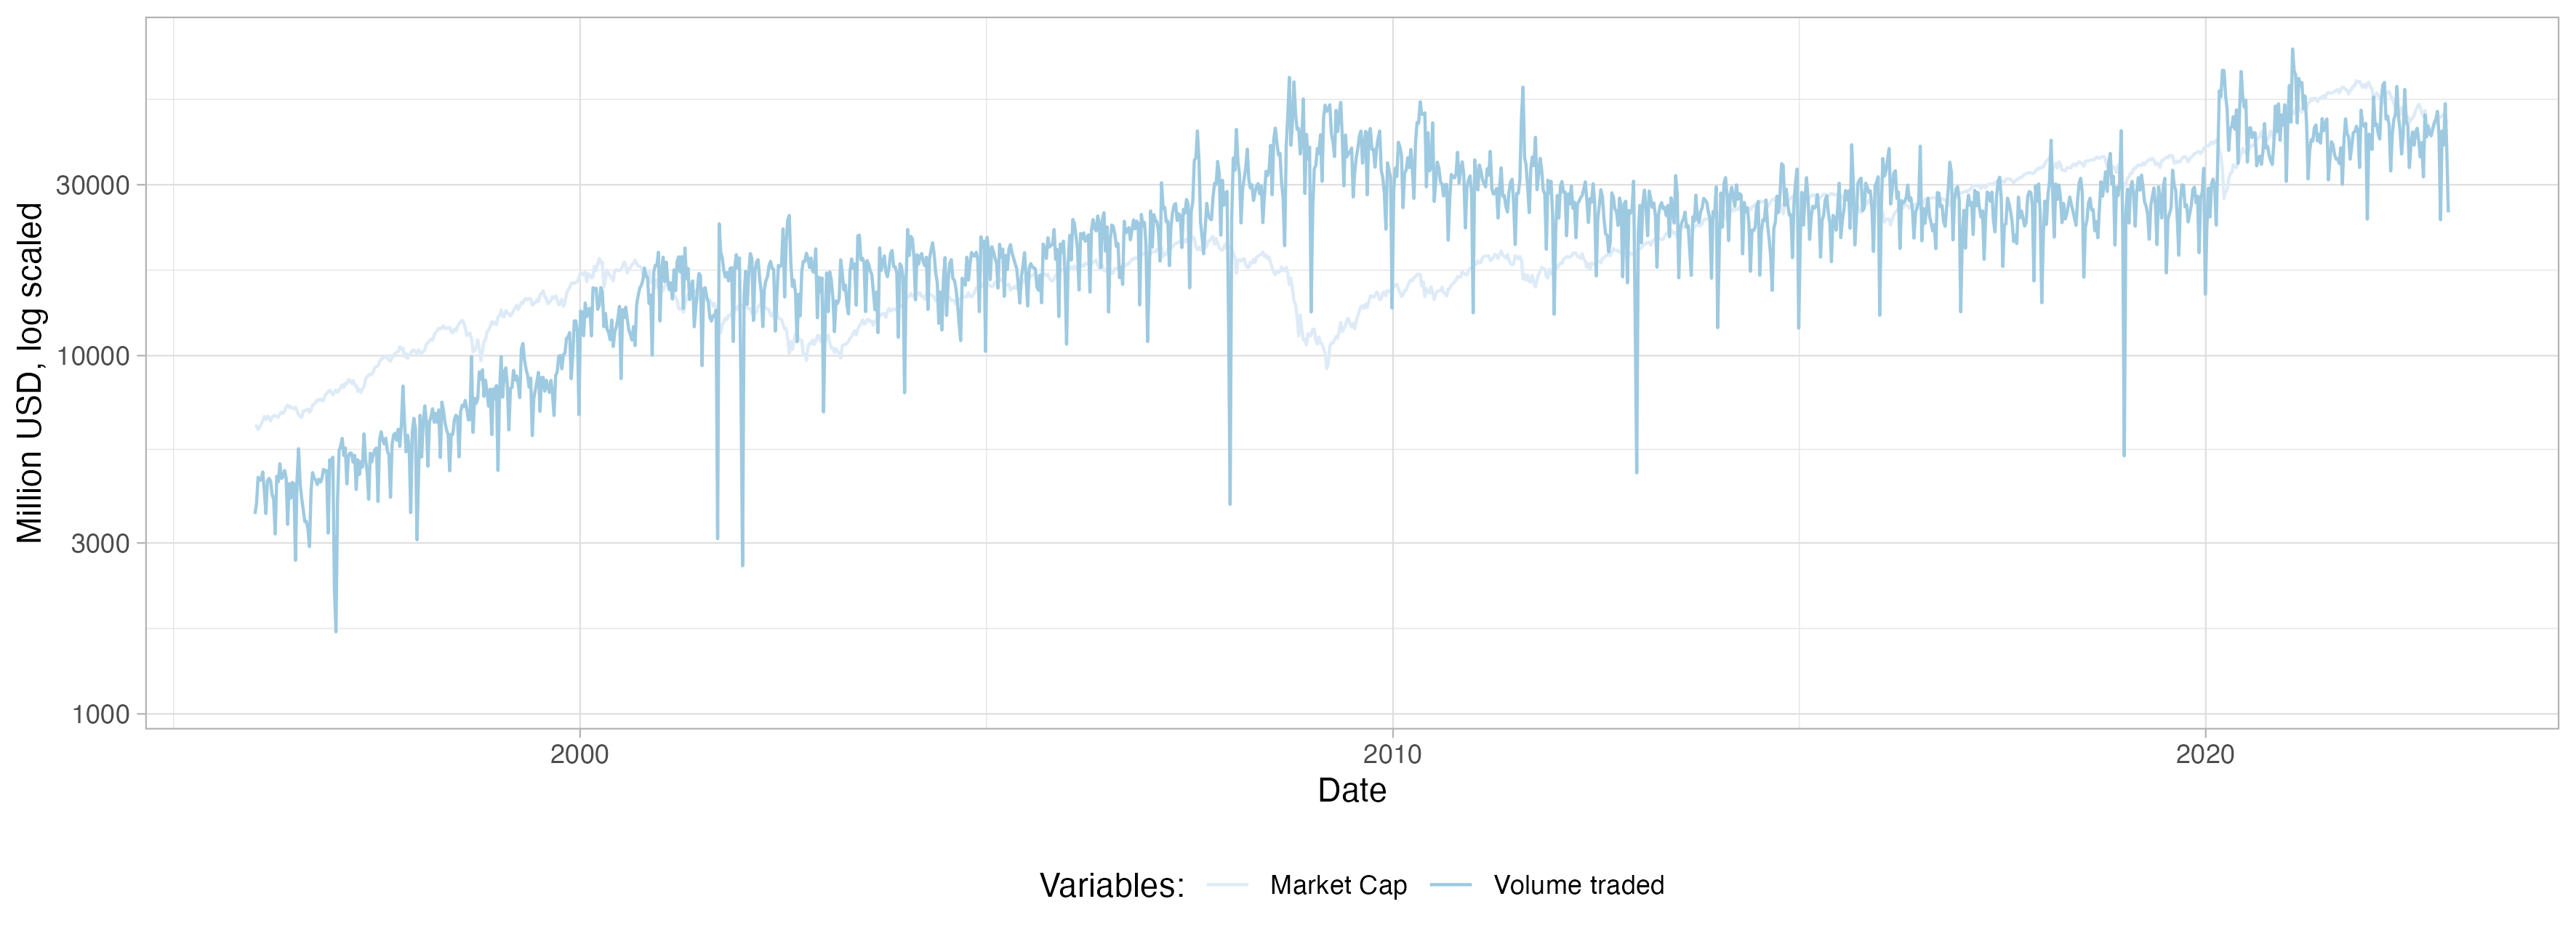
\includegraphics[width=0.85\textwidth]{./Plots/metadata_crsp_volumemarket_entireperiod.png}} \\
		\subfloat[CRSP : Number of Firms]{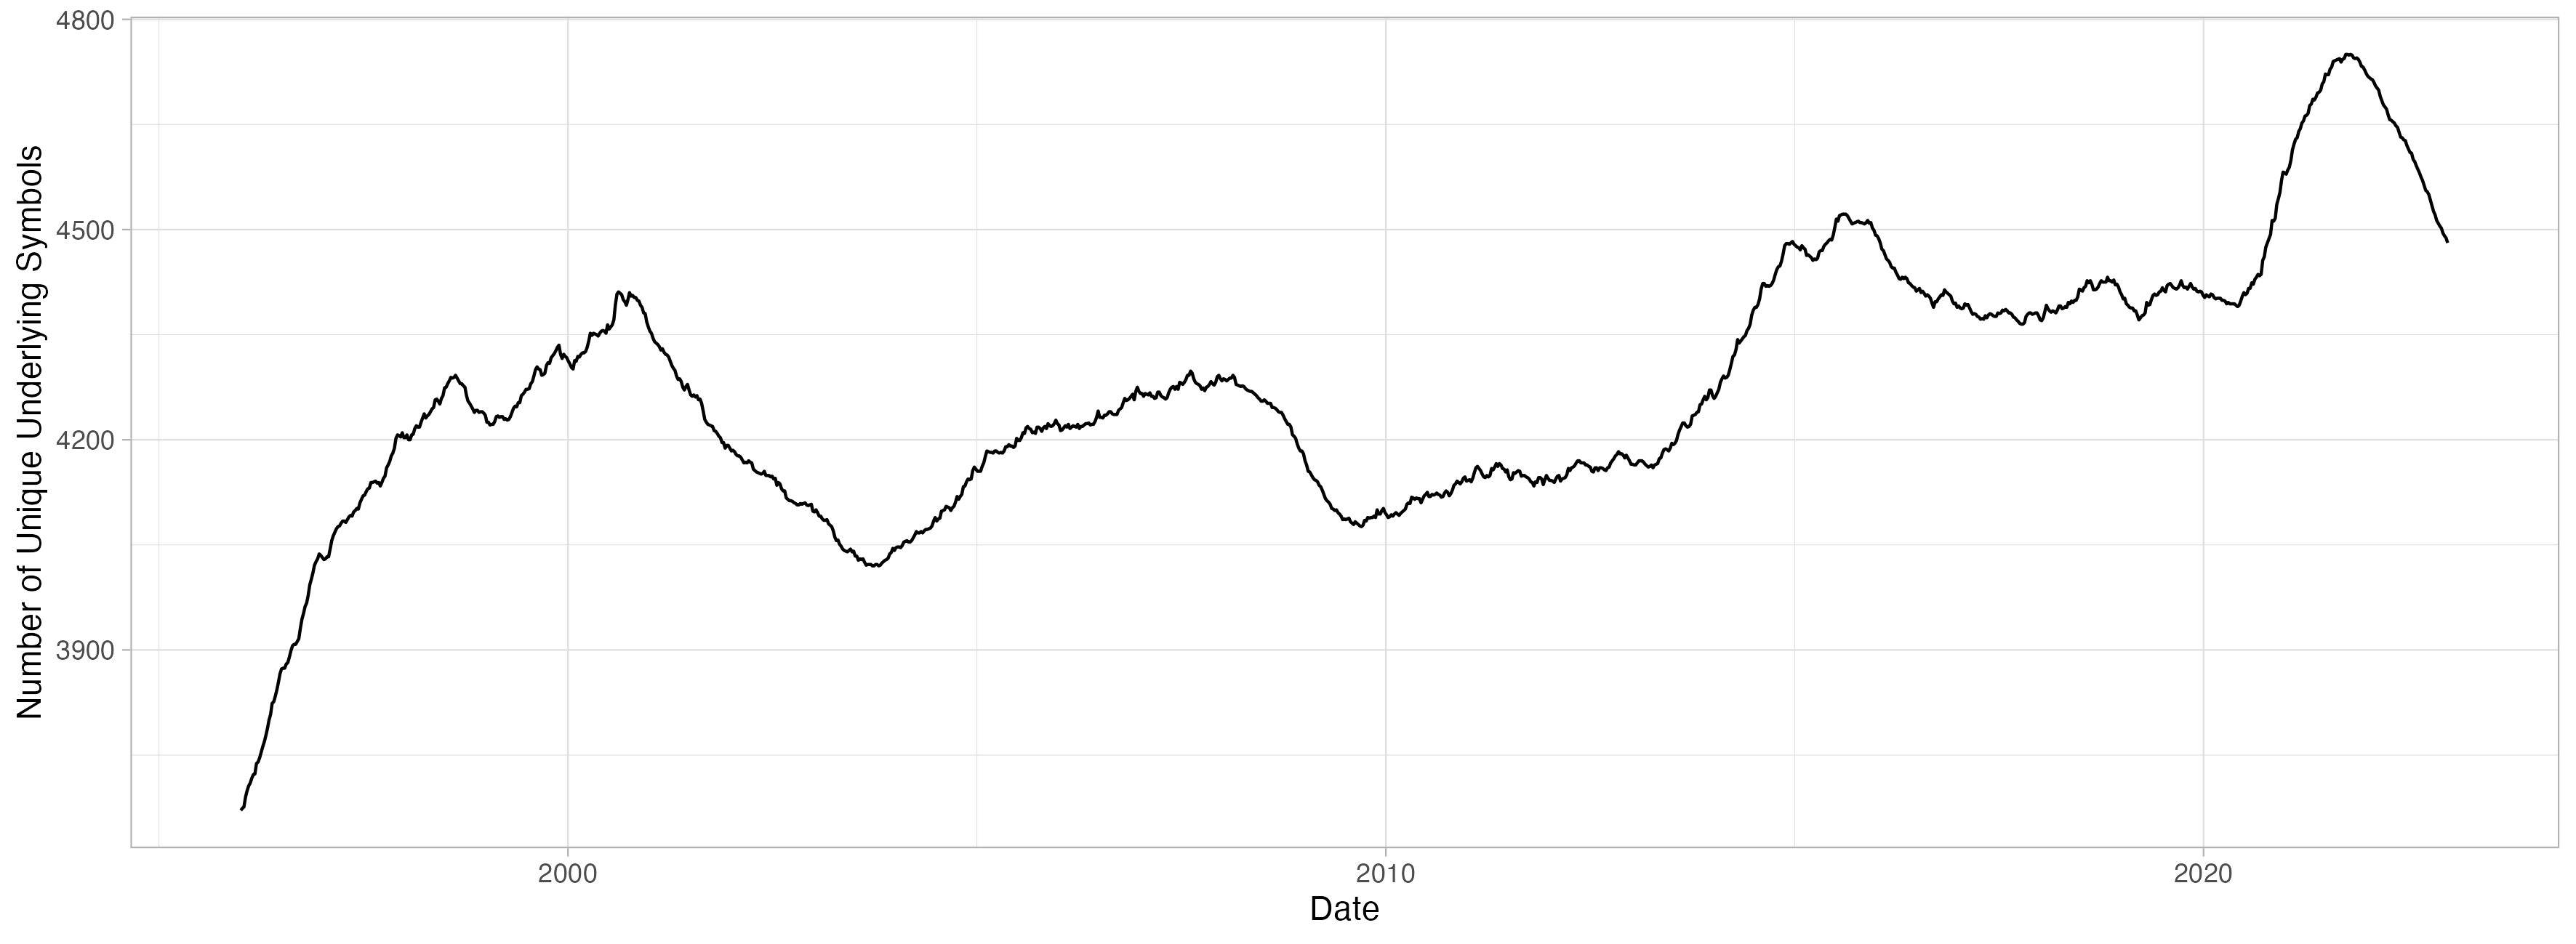
\includegraphics[width=0.85\textwidth]{./Plots/metadata_crsp_firms_entireperiod.png}} \\
		%\subfloat[CRSP : Median Bid-ask Spread]{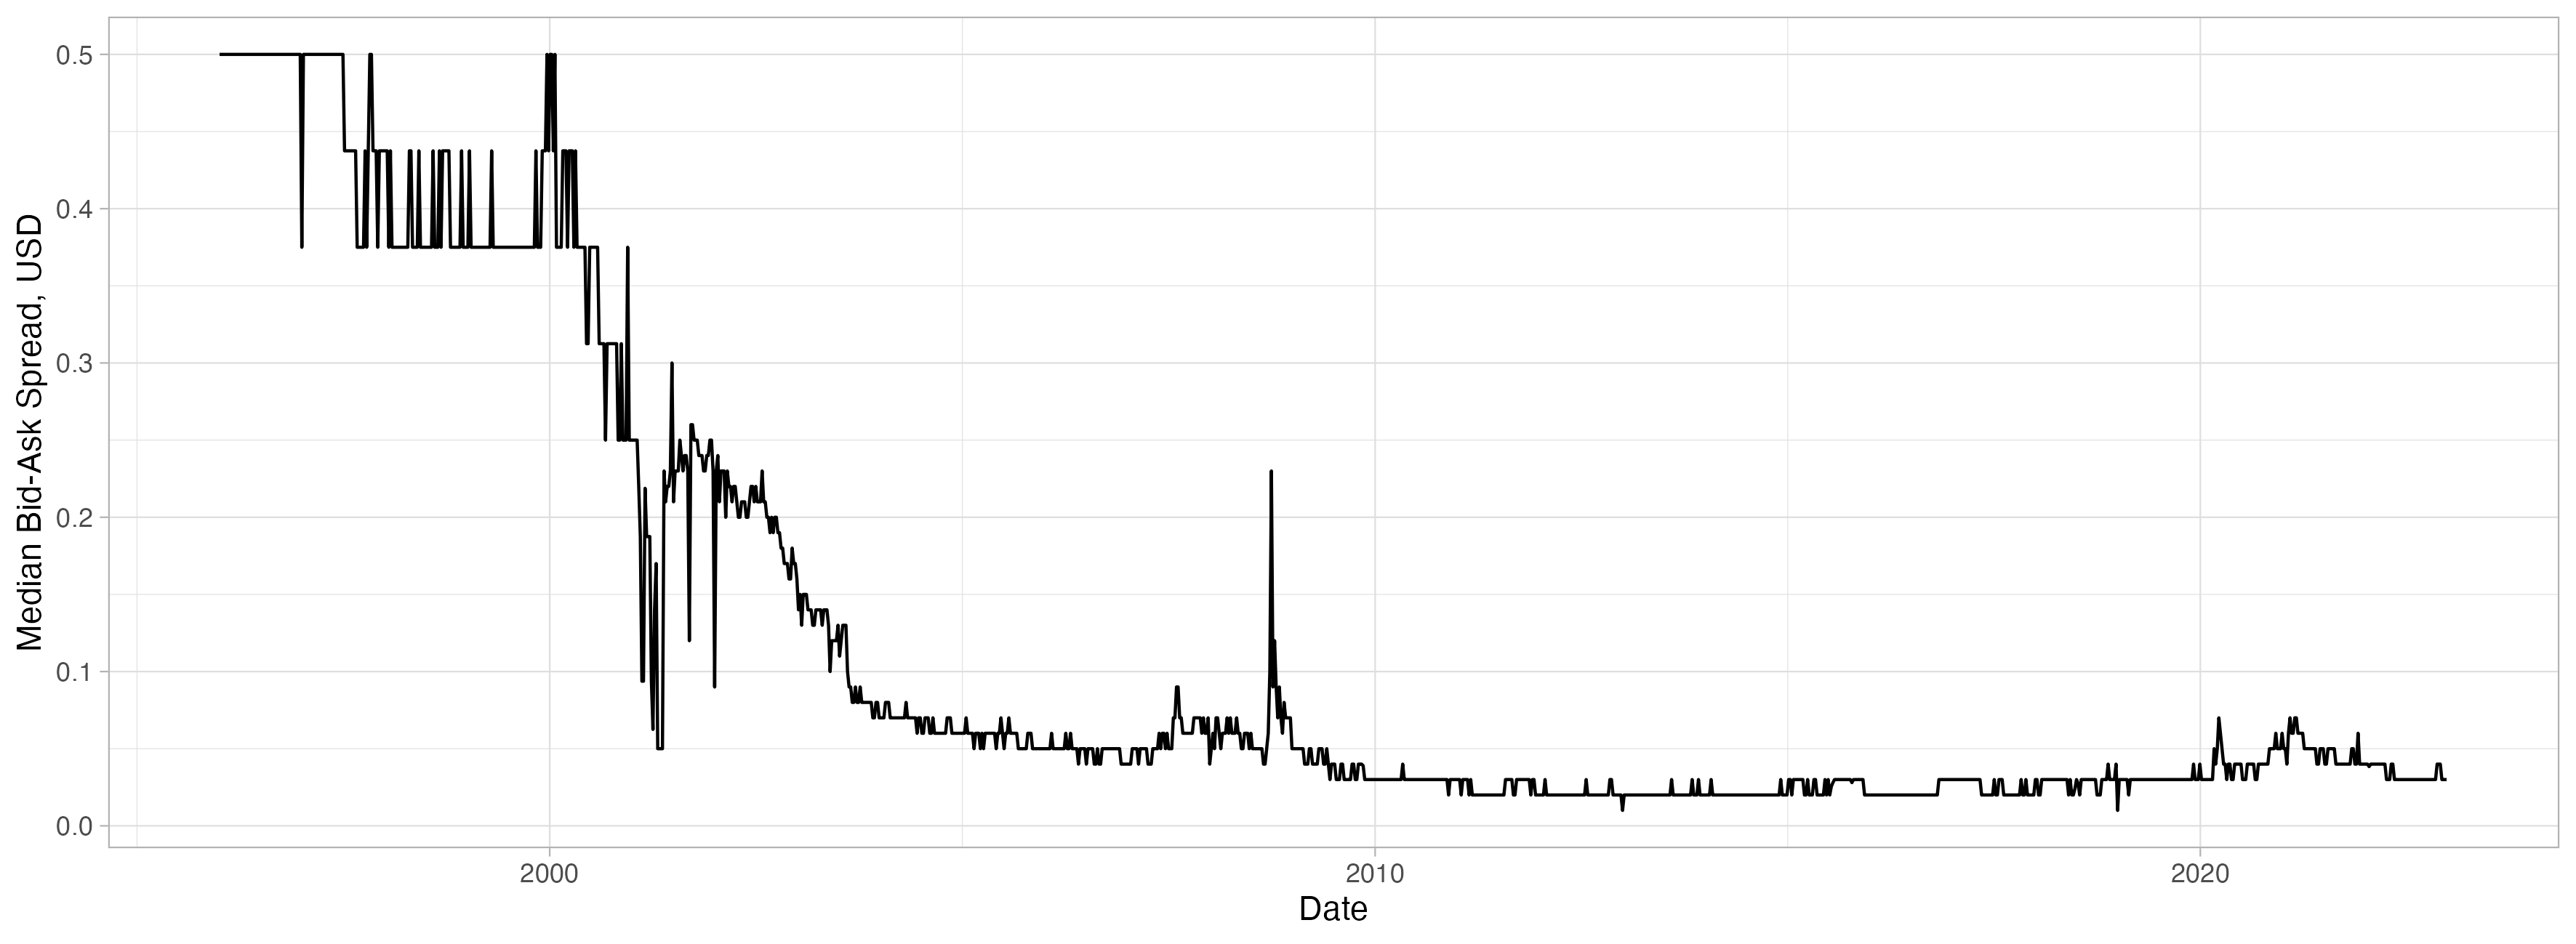
\includegraphics[width=0.6\textwidth]{./Plots/metadata_crsp_bidask_entireperiod.png}} \\
	\end{tabular}
	\label{fig:data_metadata}
	
	{\small Note: Figure shows different measures of metadata for both CRSP data and OptionMetrics data. The two subsampled in subplot (A) consist of a subsample with the conditions mentioned above imposed, and another subsample without these restrictions imposed. Note plot (B) has a log scaled Y axis.}
\end{figure}

\textbf{Other Use of Available Data} If time, scope and focus had allowed it, I would also have loved to deploy the ratio of open interest in the stock market versus the open interest in the option market. This could have been a relevant proxy for the market liquidity and how well the market prices resembled the market's beliefs. This could have been done through just a simple continuous variable which could factor in through interaction terms with the dummies of the different portfolios, and it could also be incorporated through a split into different 'levels', with the sample splitted into five subsamples resembling the five different formalized levels of the ratio. In addition to this, it could be relevant to factor in a de-trending of this ratio, to not make the earliest years with very few options offered constitute the lowest group. 